\documentclass{article}
\usepackage[preprint]{neurips_2025}
\usepackage[utf8]{inputenc}
\usepackage[T1]{fontenc}
\usepackage{amsmath,amssymb,booktabs,graphicx,url,hyperref}
\hypersetup{colorlinks=true,citecolor=blue,linkcolor=blue,urlcolor=blue}
\newcommand{\soft}{\mathcal{S}}
\newcommand{\R}{\mathbb{R}}
\title{ISTA, FISTA, and ADMM for Sparse Linear Regression:\\An Empirical Comparison with Certified Stopping}
\author{}
\makeatletter
\renewcommand{\@noticestring}{Source code and reproducibility materials: \href{https://github.com/Yuchen-Wang-CHN/comp6704-lasso-optimization}{GitHub repository}.}
\makeatother
\begin{document}
\maketitle
\begin{abstract}
Optimization comparisons for LASSO depend on stopping accuracy and implementation costs as well as theoretical convergence rates. This project implements ISTA, FISTA, ADMM, and FISTA with an established gradient-based adaptive restart rule. A common feasible primal--dual certificate controls accuracy, while ADMM additionally satisfies primal and dual residual criteria. Across 710 runs covering synthetic data and the UCI Online News Popularity dataset, every method reaches a relative dual gap below $10^{-6}$. In the baseline Gram-matrix implementation, restarted FISTA has the lowest mean total runtime on both datasets. A further 40 direct-matrix runs reverse the leading ranking: ADMM is fastest when proximal-gradient methods repeatedly traverse the full data matrix. Regularization and data splitting affect prediction and feature selection much more than the choice of a converged solver. These results establish the linear-algebra backend and setup cost as practical criteria for algorithm selection in dense LASSO problems.
\end{abstract}

\section{Introduction}
Sparse linear regression combines squared-error fitting with an $\ell_1$ penalty to estimate a predictive model with relatively few active coefficients. The resulting LASSO objective is convex, but the absolute-value penalty is not differentiable at zero. Proximal-gradient methods and splitting methods exploit this structure without requiring a smooth approximation to the penalty.

The iterative shrinkage-thresholding algorithm (ISTA), its accelerated form FISTA, and the alternating direction method of multipliers (ADMM) take substantially different routes to the same solution. Standard objective-value bounds favor FISTA over ISTA in the general convex setting. These bounds do not determine the fastest implementation at a prescribed numerical accuracy: setup work, linear algebra, diagnostics, and data dimensions also matter. Momentum can also produce oscillatory objective trajectories, motivating adaptive restart.

This study asks which method reaches a common accuracy fastest, how sample and feature counts affect runtime, how regularization affects prediction and sparsity, how results vary with noise and feature correlation, and whether adaptive restart improves FISTA. The contribution is a reproducible controlled comparison of established methods, with explicit timing boundaries and a backend sensitivity check.

\section{Related work}
Tibshirani introduced the LASSO as a regression and variable-selection procedure \citep{tibshirani1996}. Its non-smooth penalty has a simple proximal map, making the objective suitable for first-order composite optimization. Beck and Teboulle developed FISTA and established an accelerated objective-value bound while preserving the basic proximal-gradient operation \citep{beck2009}. The present comparison connects these objective-value rates with measured time to certified accuracy.

ADMM introduces auxiliary variables to separate subproblems. The survey of \citet{boyd2011} describes LASSO updates, cached factorization, convergence conditions, and residual stopping criteria. These considerations motivate reporting setup and iteration costs separately. O'Donoghue and Cand\`es proposed adaptive restart for accelerated schemes, including a generalized-gradient restart test for sparse regression \citep{odonoghue2015}. More recent analysis establishes guarantees for a gradient-restart strategy in settings including one-dimensional functions \citep{moursi2023}. Here, paired runs measure the effect of restart on time to certified accuracy.

\section{Problem formulation and algorithms}
\subsection{A shared LASSO objective}
For a training matrix $X\in\R^{n\times d}$ and centered target $y\in\R^n$, all solvers minimize
\begin{equation}
 F(w)=f(w)+g(w)=\frac{1}{2n}\|Xw-y\|_2^2+\lambda\|w\|_1,\qquad \lambda>0.
 \label{eq:objective}
\end{equation}
Training features are centered and scaled to unit population standard deviation, using training statistics only. Constant columns receive scale one. The target is centered without variance scaling. If $\mu_X$, $s_X$, and $\mu_y$ denote the fitted means and scales, raw coefficients and the unpenalized intercept are $w_{\rm raw}=w/s_X$ and $b=\mu_y-\mu_X^T w_{\rm raw}$.

The gradient and its Lipschitz constant are
\begin{equation}
 \nabla f(w)=X^T(Xw-y)/n=Gw-q,\qquad L=\|X\|_2^2/n,
\end{equation}
where $G=X^TX/n$ and $q=X^Ty/n$. The soft-thresholding map is
$[\soft_a(v)]_j=\operatorname{sign}(v_j)\max(|v_j|-a,0)$.
The subgradient interval of $|w_j|$ at zero permits an optimum with $w_j=0$ when the corresponding loss gradient is sufficiently small. In particular, the zero vector is optimal for $\lambda\geq\lambda_{\max}=\|q\|_\infty$.

\subsection{ISTA and FISTA}
Starting from $w^0=0$, ISTA uses
\begin{equation}
 w^{k+1}=\soft_{\lambda/L}\bigl(w^k-\nabla f(w^k)/L\bigr).
\end{equation}
The implementation computes the largest eigenvalue of $G$ for the Gram backend, or the largest singular value of $X$ for the direct backend. A factor $1+10^{-12}$ increases the computed Lipschitz constant slightly to guard against rounding. This calculation is charged to the method's setup time.

FISTA starts with $v^0=w^0$ and $t_0=1$ and performs
\begin{align}
 w^{k+1}&=\soft_{\lambda/L}\bigl(v^k-\nabla f(v^k)/L\bigr),\\
 t_{k+1}&=(1+\sqrt{1+4t_k^2})/2,\\
 v^{k+1}&=w^{k+1}+\frac{t_k-1}{t_{k+1}}(w^{k+1}-w^k).
\end{align}
For convex $f$ with $L$-Lipschitz gradient, proper closed convex $g$, an attained minimum, and this step size, the standard bounds are
\begin{equation}
 F(w^k)-F^*\leq\frac{L\|w^0-w^*\|^2}{2k}\quad\text{(ISTA)},\qquad
 F(w^k)-F^*\leq\frac{2L\|w^0-w^*\|^2}{(k+1)^2}\quad\text{(FISTA)}.
\end{equation}
These bounds quantify objective-error decay. The experiments measure the corresponding elapsed time to the prescribed dual-gap threshold.

The restart variant tests $(v^k-w^{k+1})^T(w^{k+1}-w^k)>0$. When the test holds, it retains $w^{k+1}$, resets the next momentum parameter to one, and sets the next extrapolated point to $w^{k+1}$. Otherwise it uses the standard FISTA update. This is the established generalized-gradient restart rule \citep{odonoghue2015}.

\subsection{ADMM}
Introducing $z$ gives $\min_{w,z} f(w)+\lambda\|z\|_1$ subject to $w=z$. With scaled dual variable $u$ and fixed $\rho>0$,
\begin{align}
 (G+\rho I)w^{k+1}&=q+\rho(z^k-u^k),\\
 z^{k+1}&=\soft_{\lambda/\rho}(w^{k+1}+u^k),\\
 u^{k+1}&=u^k+w^{k+1}-z^{k+1}.
\end{align}
One Cholesky factorization is cached per solve; explicit matrix inversion is avoided. The reported coefficients are $z$, and its unsplit objective in Equation~\ref{eq:objective} is used for comparisons. The primal and dual residual norms are
$r_k=\|w^k-z^k\|_2$ and $s_k=\rho\|z^k-z^{k-1}\|_2$.
Their thresholds are
\begin{align}
 \epsilon_{\rm pri}&=\sqrt{d}\,10^{-6}+10^{-5}\max(\|w^k\|_2,\|z^k\|_2),\\
 \epsilon_{\rm dual}&=\sqrt{d}\,10^{-6}+10^{-5}\|\rho u^k\|_2.
\end{align}
The loss and penalty are closed proper convex functions, a solution exists for $\lambda>0$, and the equality split has full-rank identity constraint blocks. Fixed positive $\rho$ and exact subproblem solves give the applicable ADMM convergence setting \citep{boyd2011}.

\subsection{A common stopping certificate}
For $r=y-Xw$, set
\begin{equation}
 \theta=\frac{a r}{n},\qquad
 a=\min\left(1,\frac{\lambda}{\|X^Tr/n\|_\infty}\right).
\end{equation}
If the correlation norm is zero, take $a=1$; the implementation moves nontrivial scaling a negligible amount inward for numerical feasibility. Then $\|X^T\theta\|_\infty\leq\lambda$, so the dual objective
\begin{equation}
 D(\theta)=y^T\theta-\frac{n}{2}\|\theta\|_2^2
\end{equation}
is a valid lower bound, and $0\leq F(w)-F^*\leq F(w)-D(\theta)$ in exact arithmetic. All solvers stop when
\begin{equation}
 \frac{F(w)-D(\theta)}{\max(1,|F(w)|)}\leq10^{-6}.
 \label{eq:stopping}
\end{equation}
ADMM must also pass both residual tests. Certificates are checked at initialization, every five iterations, and at the 20,000-iteration limit; a limit exit is recorded as failure. Gram certificates are independently recomputed from $X$ and $y$ at the endpoint to detect cancellation. A scikit-learn coordinate-descent reference uses the identical objective with \texttt{alpha=lambda}, \texttt{fit\_intercept=False}, tolerance $10^{-12}$, and a separately checked direct relative dual gap below $10^{-9}$ \citep{sklearnlasso}. Objective differences to this numerical reference are reported separately from the certified dual gap.

\section{Experimental design}
\subsection{Datasets and splits}
Synthetic features have unit-variance Gaussian AR(1) correlation, $\operatorname{Cov}(X_i,X_j)=c^{|i-j|}$. The generator recursively sets $X_j=cX_{j-1}+\sqrt{1-c^2}\,E_j$ from independent standard-normal columns. A uniformly selected support has $\max(1,\operatorname{round}(pd))$ active coefficients, random signs, and magnitudes uniform on $[0.5,2]$. Targets are $y=2+Xw^*+\varepsilon$ with $\varepsilon\sim N(0,\sigma^2I)$. Baseline settings are 5,000 total samples, 200 features, $p=0.1$, $c=0.9$, and $\sigma=1$.

Online News Popularity contains 39,644 observations and 58 predictors after removing the non-predictive \texttt{url} and \texttt{timedelta} columns \citep{uci2015}. The target is $\log(1+\mathrm{shares})$. All rows and all 58 predictors are retained, and the loader checks for missing and nonfinite values. The official archive and extracted CSV have recorded SHA-256 hashes and attribution under CC BY 4.0.

Each seed in $\{0,1,2,3,4\}$ determines a 70/15/15 random train/validation/test split. The baseline synthetic split has 3,500/750/750 rows, and the news split has 27,750/5,947/5,947. Feature scaling and target centering use the training portion only. The same matrices, zero initialization, and regularization are used for every method within each case. Synthetic seeds change the generated data and true coefficients; news seeds change only the split. Seed-level summaries describe this data/split variability.

\subsection{Experiment matrix}
The main study contains 200 cases and 710 solver runs:
\begin{center}
\small
\begin{tabular}{llr}
\toprule
Experiment & Variation & Solver runs\\
\midrule
Baseline convergence & Two datasets, five seeds, $\lambda/\lambda_{\max}=0.03$ & 40\\
Sample scaling & $n_{\rm total}\in\{1000,5000,20000\}$, $d=200$ & 60\\
Feature scaling & $d\in\{50,200,500\}$, $n_{\rm total}=5000$ & 60\\
Regularization & Seven ratios, two datasets, five seeds & 280\\
Robustness & Three noise levels, two correlations, two sparsities & 240\\
ADMM penalty & $\rho\in\{0.1,1,10\}$, two datasets, five seeds & 30\\
\bottomrule
\end{tabular}
\end{center}
The penalty ratios are $\{1,0.3,0.1,0.03,0.01,0.003,0.001\}$.
Robustness varies $\sigma\in\{0.1,1,3\}$, $c\in\{0.1,0.9\}$, and $p\in\{0.05,0.1\}$ at the baseline dimensions. ADMM uses $\rho=1$ outside its sensitivity sweep. Scaling varies one factor at a time. Forty additional direct-backend baseline runs test implementation dependence.

For prediction, one regularization ratio per dataset and seed is selected by the reference model's validation MSE. Every custom solver is then evaluated at that shared selected ratio on the test set. Test MSE is computed only after selection, using the models fitted on the original 70\% training partition. Nonzero counts use $|w_j|>10^{-6}$. Synthetic coefficient error is measured after converting coefficients to raw-feature units, and support F1 compares estimated and known supports.

\subsection{Timing, storage, and uncertainty}
Experiments run in float64 on Windows 11 with an Intel Core i7-14700 processor. Numerical thread pools are limited to one thread. The environment records Python 3.12.14, NumPy 2.5.4, SciPy 1.18.1, pandas 3.1.0, scikit-learn 1.9.1, and Matplotlib 3.11.2; a full dependency lock and BLAS metadata accompany the outputs. Numerical kernels are warmed before timing and solver order is deterministically shuffled within each case.

The main backend precomputes $G$ and $q$. Its measured common construction cost is charged to every method, even when the matrix is physically reused between solver calls. Each method additionally pays its own setup and iteration costs, including certificate evaluation and history recording. Split/standardization time is recorded separately; data acquisition, reference optimization, prediction, and disk I/O are excluded from optimization time. In the direct backend, proximal-gradient gradients and certificates use $X$, and exact SVD-based step-size setup is charged to each method. Direct ADMM constructs its own $G$ and factors $G+\rho I$ within setup.

Gram construction costs $O(nd^2)$ time and $O(d^2)$ additional storage; cached proximal-gradient iterations cost $O(d^2)$, compared with $O(nd)$ direct gradients. ADMM's dense factorization costs $O(d^3)$, followed by $O(d^2)$ triangular solves. Reported storage is the analytic size of the allocated data and Gram arrays. All mean $\pm$ SD summaries use sample standard deviation across the stated seeds or configurations.

\section{Results and analysis}
\subsection{Certified convergence and the value of restart}
All 710 main-study runs and all 40 direct-backend runs meet their stopping rules. Across these 750 endpoints, the largest directly verified relative dual gap is $9.9993\times10^{-7}$. The largest absolute objective difference from the coordinate-descent reference is $3.3311\times10^{-10}$, and the largest relative training-prediction disagreement is $9.0665\times10^{-5}$. Every ADMM endpoint also satisfies both residual checks. These comparisons support implementation correctness at the tested accuracy, including cases in which coefficients need not be unique.

\begin{table}[t]
\centering\scriptsize
\begin{tabular}{llrrrr}
\toprule
Data & Method & Iterations & Total (ms) & Setup (ms) & Nonzeros \\
\midrule
Synthetic & ISTA & 3528 $\pm$ 312 & 51.09 $\pm$ 12.95 & 0.80 $\pm$ 0.27 & 28.4 $\pm$ 3.0 \\
Synthetic & FISTA & 2445 $\pm$ 158 & 38.13 $\pm$ 4.29 & 0.65 $\pm$ 0.06 & 28.4 $\pm$ 3.0 \\
Synthetic & Restarted FISTA & 310 $\pm$ 25 & 8.41 $\pm$ 0.83 & 0.66 $\pm$ 0.04 & 28.4 $\pm$ 3.0 \\
Synthetic & ADMM & 197 $\pm$ 24 & 13.18 $\pm$ 2.53 & 0.24 $\pm$ 0.08 & 28.4 $\pm$ 3.0 \\
News & ISTA & 891 $\pm$ 182 & 11.78 $\pm$ 2.31 & 0.20 $\pm$ 0.03 & 39.4 $\pm$ 1.5 \\
News & FISTA & 422 $\pm$ 97 & 8.69 $\pm$ 1.95 & 0.17 $\pm$ 0.01 & 39.4 $\pm$ 1.5 \\
News & Restarted FISTA & 121 $\pm$ 24 & 5.94 $\pm$ 1.34 & 0.17 $\pm$ 0.02 & 39.4 $\pm$ 1.5 \\
News & ADMM & 171 $\pm$ 8 & 8.12 $\pm$ 1.13 & 0.08 $\pm$ 0.02 & 39.4 $\pm$ 1.5 \\
\bottomrule
\end{tabular}

\caption{Baseline results at $\lambda/\lambda_{\max}=0.03$: mean $\pm$ sample SD over five seeds. Total time includes common sufficient-statistic construction, method setup, and iterations. Setup here is method-specific and excludes the separately charged common construction cost. Nonzero counts use a $10^{-6}$ threshold.}
\label{tab:baseline}
\end{table}

Restarted FISTA has the lowest mean total time in the Gram baseline: 8.41 ms on synthetic data and 5.94 ms on news (Table~\ref{tab:baseline}). ADMM requires fewer synthetic iterations, 197 versus 310 for restarted FISTA, but takes more elapsed time because an iteration contains different work. Standard FISTA reduces mean iteration counts relative to ISTA but remains slower than the restarted variant in both baseline settings.

\begin{figure}[t]
\centering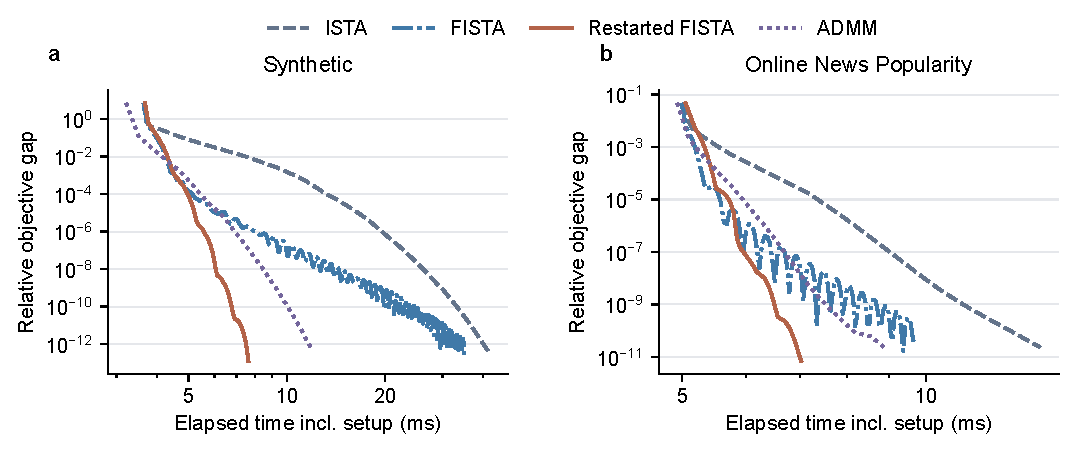
\includegraphics[width=\linewidth]{figures/02_gap_time.pdf}
\caption{Relative objective error against the high-accuracy reference versus elapsed optimization time, including setup. Panels show synthetic data (a) and news (b), both at seed 0 and penalty ratio 0.03. The plotted error is $(F(w)-F_{\rm ref})/\max(1,|F_{\rm ref}|)$; stopping uses the different, certified dual gap in Equation~\ref{eq:stopping}. Raw checkpoint values are plotted, without smoothing. Nonpositive reference differences are omitted only from logarithmic display and retained in source data.}
\label{fig:gap}
\end{figure}

The seed-0 trajectories show oscillatory objective error for standard FISTA and a faster late-stage decrease with restart (Figure~\ref{fig:gap}). Paired total-runtime ratios under the Gram backend, computed within the same dataset and seed, favor restart over FISTA by 4.22--4.99 times on the baseline synthetic problem and 1.38--1.54 times on news. The dual-gap certificate controls termination even after the objective is very close to the reference, connecting the observed runtime advantage to a shared accuracy target.

\begin{figure}[t]
\centering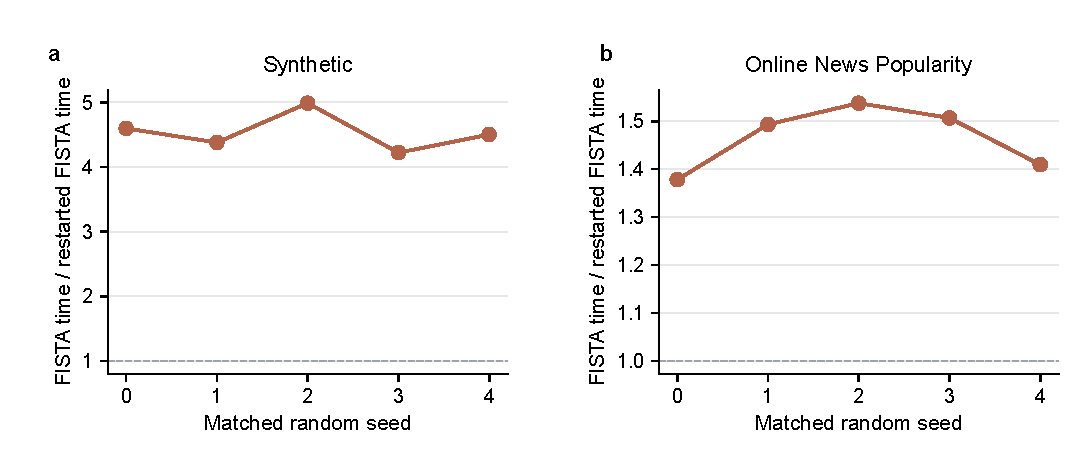
\includegraphics[width=\linewidth]{figures/05_restart_paired.pdf}
\caption{Paired runtime benefit of adaptive restart in the Gram baseline. Each point is FISTA total time divided by restarted FISTA total time for the same dataset, seed, and penalty ratio 0.03. Panels show synthetic data (a) and news (b). The dashed line marks equal runtime; every observed pair favors restart.}
\label{fig:restart}
\end{figure}

Figure~\ref{fig:restart} extends the trajectory comparison to all five seeds per dataset. The mean paired speedup is $4.54\pm0.29$ on synthetic data and $1.46\pm0.07$ on news, with sample SD across seeds. Pairing holds the generated problem or data split fixed within each ratio, so the comparison directly tracks the effect of resetting momentum. Restarted FISTA averages 4.6 momentum resets on synthetic data and 2.8 on news. These few resets accompany reductions from 2,445 to 310 mean iterations and from 422 to 121, respectively, linking the runtime benefit to a shorter trajectory toward the common certificate.

\subsection{Sample scaling, feature scaling, and backend dependence}
Increasing the number of samples has a different cost profile from increasing the number of features (Figure~\ref{fig:scale}). Once the Gram matrix is available, an iteration operates on feature-sized sufficient statistics. Sample growth primarily increases common construction cost, whereas feature growth affects common construction, spectral setup, matrix-vector products, and ADMM factorization. This division of work explains the comparatively flat sample-scaling curves for the slower iterative methods.

\begin{figure}[t]
\centering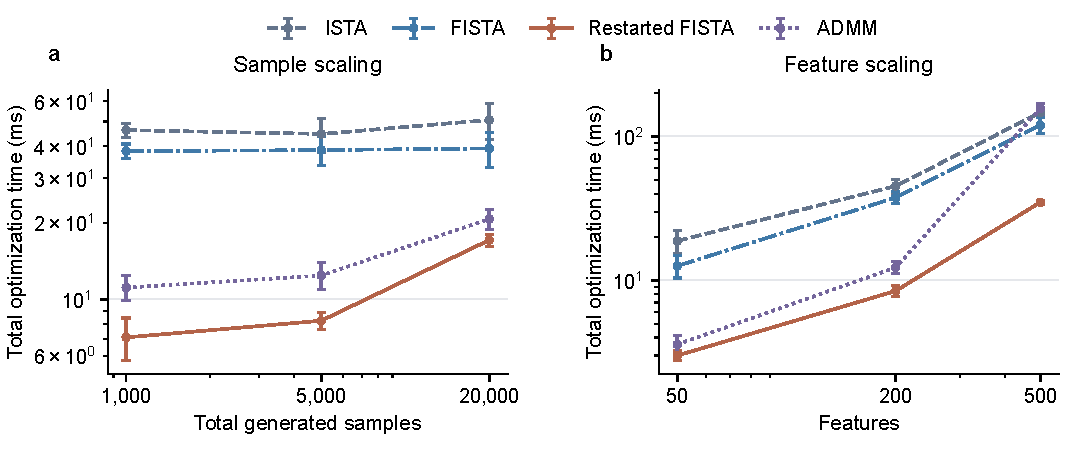
\includegraphics[width=\linewidth]{figures/03_scalability.pdf}
\caption{Total optimization time versus total generated sample count at $d=200$ (a), and feature count at 5,000 total samples (b). Training uses 70\% of the generated samples. Points show means and error bars show sample SD over five seeds. All methods use the Gram backend and include construction and method setup.}
\label{fig:scale}
\end{figure}

\begin{table}[t]
\centering\small
\begin{tabular}{llrr}
\toprule
Data & Method & Gram total (ms) & Direct total (ms) \\
\midrule
Synthetic & ISTA & 51.09 $\pm$ 12.95 & 628.41 $\pm$ 52.17 \\
Synthetic & FISTA & 38.13 $\pm$ 4.29 & 443.05 $\pm$ 24.54 \\
Synthetic & Restarted FISTA & 8.41 $\pm$ 0.83 & 73.24 $\pm$ 4.91 \\
Synthetic & ADMM & 13.18 $\pm$ 2.53 & 19.28 $\pm$ 1.66 \\
News & ISTA & 11.78 $\pm$ 2.31 & 589.15 $\pm$ 125.86 \\
News & FISTA & 8.69 $\pm$ 1.95 & 298.32 $\pm$ 77.24 \\
News & Restarted FISTA & 5.94 $\pm$ 1.34 & 106.03 $\pm$ 15.62 \\
News & ADMM & 8.12 $\pm$ 1.13 & 28.34 $\pm$ 2.64 \\
\bottomrule
\end{tabular}

\caption{Baseline runtime sensitivity to linear-algebra backend: mean $\pm$ sample SD over the same five seeds. Both columns measure complete implementations, including backend-specific setup, iterations, and diagnostics.}
\label{tab:backend}
\end{table}

The direct-backend experiment reverses the leading runtime ranking (Table~\ref{tab:backend}). ADMM averages 19.28 ms on synthetic data and 28.34 ms on news, compared with 73.24 and 106.03 ms for restarted FISTA. Its cached factorization avoids a full data traversal on every iteration, while the direct proximal-gradient methods repeatedly multiply by $X$ and $X^T$. Their exact SVD-based Lipschitz setup is also more expensive than the Gram eigenvalue calculation. The iteration counts match the corresponding Gram runs, isolating a large implementation effect even when the optimization trajectory is essentially unchanged. The fastest tested method therefore depends on backend and setup choices.

\paragraph{Connecting iteration savings to total runtime.}
For method $m$, the recorded optimization time can be written as
\begin{equation}
 T_m=C+S_m+K_m\bar{c}_m,
 \label{eq:cost}
\end{equation}
where $C$ is common construction time, $S_m$ is method setup, $K_m$ is the iteration count, and $\bar{c}_m$ is measured iteration-phase time divided by $K_m$, including diagnostics. This accounting connects the iteration trajectories to the end-to-end comparisons. Adaptive restart acts primarily through $K_m$; the backend changes both setup and the work charged to each iteration.

In the synthetic Gram baseline, restarted FISTA spends 2.96 ms on common construction, 0.66 ms on method setup, and 4.78 ms on iterations. On news, the corresponding costs are 4.34, 0.17, and 1.43 ms. Common construction plus method setup therefore accounts for 43.1\% and 75.9\% of total time, respectively, calculated as the ratio of five-seed mean costs. This larger fixed-cost share on news explains why a 3.49-fold reduction in mean iteration count translates into a 1.46-fold mean paired total-runtime speedup. The cost decomposition identifies where computational effort is spent and makes the measured restart benefit easier to transfer to an implementation decision.

\subsection{Regularization, prediction, and sparsity}
Changing the penalty changes the fitted model much more than changing a sufficiently converged solver. All methods have the same baseline nonzero counts within each seed, and their selected-model test MSE values are close (Table~\ref{tab:prediction}). The penalty sweep spans the zero model at ratio one and denser solutions at smaller ratios (Figure~\ref{fig:regularization}). Synthetic validation error increases substantially under strong shrinkage; the best tested ratios are 0.003 or 0.01 across seeds.

\begin{figure}[t]
\centering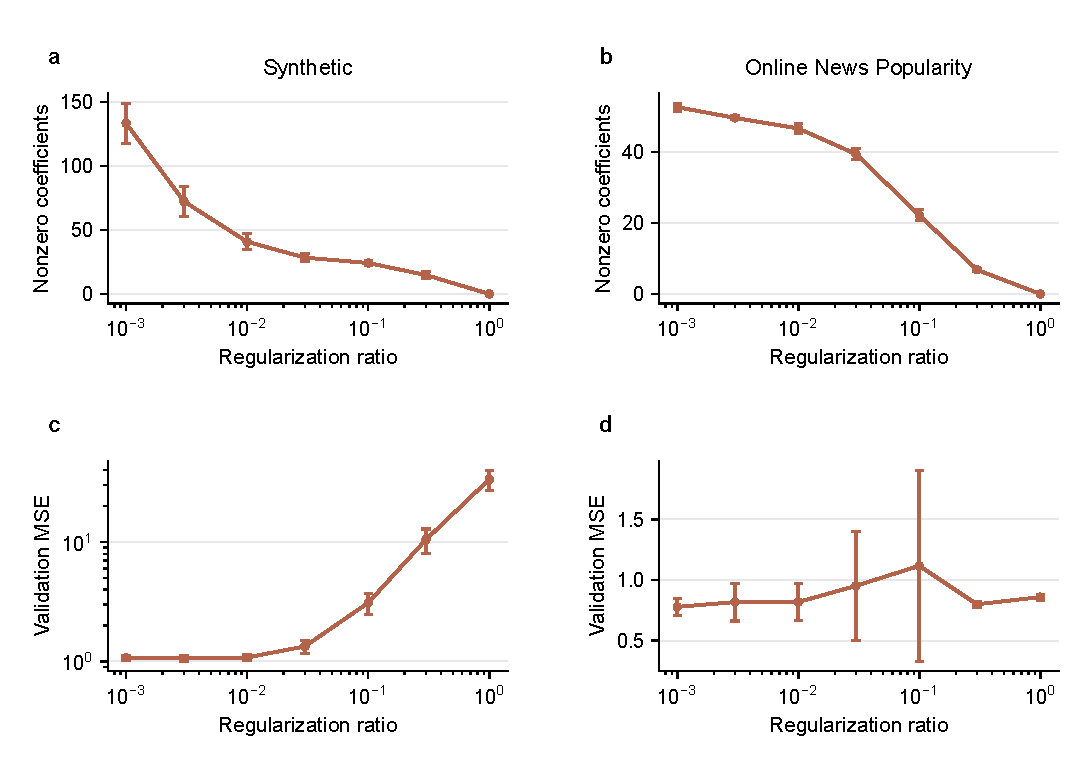
\includegraphics[width=\linewidth]{figures/04_regularization.pdf}
\caption{Regularization controls model size and validation error. Synthetic and news sparsity appear in (a,b), with corresponding validation MSE in (c,d). Points are means and error bars are sample SD over five seeds. The horizontal variable is $\lambda/\lambda_{\max}$. Restarted FISTA is displayed because all converged methods solve the same objective; all method results remain in the source CSV. Synthetic MSE uses the original target scale; news MSE uses $\log(1+\mathrm{shares})$.}
\label{fig:regularization}
\end{figure}

\begin{table}[t]
\centering\footnotesize
\begin{tabular}{llrrr}
\toprule
Data & Method & Test MSE & Test $R^2$ & Nonzeros \\
\midrule
Synthetic & ISTA & 1.0401 $\pm$ 0.0791 & 0.9652 $\pm$ 0.0082 & 63.2 $\pm$ 12.5 \\
Synthetic & FISTA & 1.0401 $\pm$ 0.0791 & 0.9652 $\pm$ 0.0082 & 63.2 $\pm$ 12.5 \\
Synthetic & Restarted FISTA & 1.0401 $\pm$ 0.0791 & 0.9652 $\pm$ 0.0082 & 63.2 $\pm$ 12.5 \\
Synthetic & ADMM & 1.0401 $\pm$ 0.0791 & 0.9652 $\pm$ 0.0082 & 63.2 $\pm$ 12.5 \\
News & ISTA & 0.7833 $\pm$ 0.0414 & 0.0822 $\pm$ 0.0574 & 40.8 $\pm$ 18.9 \\
News & FISTA & 0.7833 $\pm$ 0.0413 & 0.0823 $\pm$ 0.0572 & 40.8 $\pm$ 18.9 \\
News & Restarted FISTA & 0.7833 $\pm$ 0.0414 & 0.0822 $\pm$ 0.0573 & 40.8 $\pm$ 18.9 \\
News & ADMM & 0.7833 $\pm$ 0.0414 & 0.0822 $\pm$ 0.0574 & 40.8 $\pm$ 18.9 \\
\bottomrule
\end{tabular}

\caption{Final test results after shared validation-based penalty selection: mean $\pm$ sample SD over five splits. Each method retains its model trained on the original training partition. Synthetic MSE uses the original target scale; news MSE uses $\log(1+\mathrm{shares})$.}
\label{tab:prediction}
\end{table}

News prediction varies substantially by split. Restarted FISTA's mean test MSE is 0.7833 and mean test $R^2$ is 0.0822; seed 0 has a negative test $R^2$ of $-0.0136$. One validation split, seed 3, selects penalty ratio 0.3, whereas the others select 0.003 or 0.01. In that split, a retained \texttt{n\_non\_stop\_words} observation lies approximately 6,129 training standard deviations from the training mean. At penalty ratio 0.1, a single validation observation accounts for approximately 68.6\% of the sum of squared validation errors. These diagnostics identify the contribution of extreme feature values to the split-level validation errors and complement the solver-accuracy results.

\subsection{Robustness and ADMM penalty sensitivity}
Feature correlation strongly changes optimization difficulty in the tested synthetic settings. Across the 30 cases at correlation 0.1 (three noise levels, two sparsities, and five seeds), ISTA averages 23 iterations; at correlation 0.9 it averages 3,139. Restarted FISTA averages 17 and 278 iterations, respectively. The methods have similar coefficient-recovery metrics at a fixed problem, while increasing correlation worsens mean recovery error. Table~\ref{tab:robustness} reports the complete correlation-level comparison; its SD combines configuration differences and seed variability.

\begin{table}[t]
\centering\scriptsize
\begin{tabular}{llrrrr}
\toprule
Corr. & Method & Iterations & Total (ms) & F1 & Coef. error \\
\midrule
0.1 & ISTA & 23 $\pm$ 2 & 3.85 $\pm$ 0.21 & 0.796 & 0.056 \\
0.1 & FISTA & 30 $\pm$ 3 & 4.03 $\pm$ 0.20 & 0.796 & 0.056 \\
0.1 & Restarted FISTA & 17 $\pm$ 2 & 3.83 $\pm$ 0.21 & 0.796 & 0.056 \\
0.1 & ADMM & 28 $\pm$ 2 & 4.57 $\pm$ 0.37 & 0.796 & 0.056 \\
0.9 & ISTA & 3138 $\pm$ 565 & 42.21 $\pm$ 8.31 & 0.782 & 0.211 \\
0.9 & FISTA & 1841 $\pm$ 474 & 30.60 $\pm$ 9.33 & 0.782 & 0.211 \\
0.9 & Restarted FISTA & 278 $\pm$ 41 & 8.14 $\pm$ 1.33 & 0.782 & 0.211 \\
0.9 & ADMM & 182 $\pm$ 26 & 11.63 $\pm$ 1.45 & 0.782 & 0.211 \\
\bottomrule
\end{tabular}

\caption{Robustness aggregated over 30 cases per correlation and method. Iterations and times show mean $\pm$ sample SD across the three noise levels, two true sparsities, and five seeds. F1 is mean support-recovery F1; coefficient error is mean relative $\ell_2$ error in raw-feature units. SD summarizes variation across configurations and seeds.}
\label{tab:robustness}
\end{table}

\begin{figure}[t]
\centering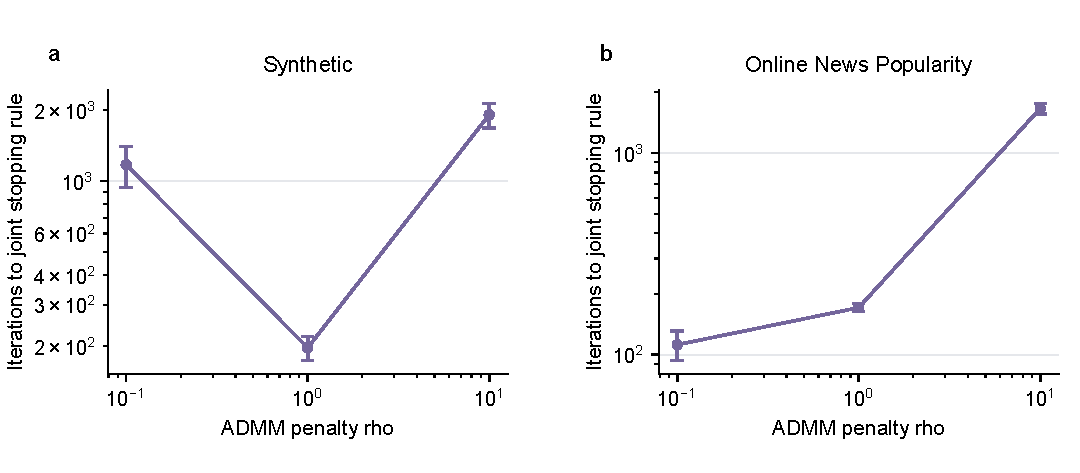
\includegraphics[width=\linewidth]{figures/06_admm_rho.pdf}
\caption{ADMM iteration counts versus fixed penalty $\rho$ for synthetic data (a) and news (b), at baseline dimensions and LASSO penalty ratio 0.03. Points show means and error bars show sample SD over five seeds. All runs require the same certified gap and both residual criteria.}
\label{fig:rho}
\end{figure}

ADMM's most efficient tested penalty differs between datasets (Figure~\ref{fig:rho}). On synthetic data, mean iterations are 1,173, 197, and 1,909 for $\rho=0.1,1,10$; on news they are 112, 171, and 1,663. The smallest mean iteration counts occur at $\rho=1$ on synthetic data and $\rho=0.1$ on news. This sweep characterizes the effect of $\rho$, while the baseline uses the shared fixed setting $\rho=1$.

For feature-selection stability, pairwise support Jaccard similarity across the five news splits is 0.833 at penalty ratio 0.03 and 0.890 at ratio 0.003 for restarted FISTA. These descriptive summaries use all ten overlapping pairs of splits. Synthetic recovery is evaluated against each seed's own true support using support F1 and coefficient error.

\section{Discussion}
The combined results distinguish optimization accuracy, computational efficiency, and statistical performance. A common certified stopping rule yields closely agreeing solutions, while the cost of reaching that accuracy depends on the work performed in each iteration and the treatment of setup. For the tested dense, moderate-dimensional problems, the backend comparison provides a concrete selection criterion: restarted FISTA is fastest with cached-Gram proximal-gradient operations, and ADMM is fastest in the direct-matrix baseline with its cached factorization.

Adaptive restart improves the baseline FISTA runtimes on both datasets. The faster late-stage decrease is consistent with the oscillation mechanism described by \citet{odonoghue2015}. Correlation and ADMM penalty sweeps further connect computational cost to problem structure and parameter choice. Together, these experiments make the case for measuring complete time to certified accuracy when selecting a solver.

The prediction experiments complement this computational comparison. Once the solvers reach the common tolerance, their fitted models agree closely; validation-based regularization and data splitting then determine the observed differences in prediction and support selection. The news diagnostics make this distinction concrete by identifying validation errors concentrated in observations with extreme feature values.

\newpage
\section{Conclusion}
The project provides original implementations, independently certified numerical endpoints, and a reproducible comparison of ISTA, FISTA, ADMM, and established adaptive-restart FISTA. Restarted FISTA achieves the lowest mean total runtime in the cached-Gram baseline, while ADMM leads the direct-matrix baseline. Algorithm selection for these dense LASSO problems should therefore consider the linear-algebra backend, setup cost, penalty setting, and required accuracy. Shared validation-based penalty selection connects the converged solutions to prediction and feature-selection outcomes.

\section*{Reproducibility}
Source code and reproducibility materials are publicly available in the \href{https://github.com/Yuchen-Wang-CHN/comp6704-lasso-optimization}{GitHub repository}.
The accompanying project contains source code, 36 passing correctness tests, configuration files, downloaded-data provenance, dependency versions, per-run histories, saved coefficients and split indices, figure source data, automated figure QA, and generated tables. Commands for reproducing the main study and direct-backend check are documented in the README. Auxiliary figures include objective versus iterations and ADMM residual trajectories. Paired speedups and timing components can be recalculated from the stored run-level CSV files. Tables are generated directly from stored CSV files.

\begin{thebibliography}{9}
\bibitem[Tibshirani(1996)]{tibshirani1996}
Robert Tibshirani. Regression shrinkage and selection via the lasso. \emph{Journal of the Royal Statistical Society: Series B}, 58(1):267--288, 1996. \url{https://doi.org/10.1111/j.2517-6161.1996.tb02080.x}.
\bibitem[Beck and Teboulle(2009)]{beck2009}
Amir Beck and Marc Teboulle. A fast iterative shrinkage-thresholding algorithm for linear inverse problems. \emph{SIAM Journal on Imaging Sciences}, 2(1):183--202, 2009. \url{https://doi.org/10.1137/080716542}.
\bibitem[Boyd et~al.(2011)]{boyd2011}
Stephen Boyd, Neal Parikh, Eric Chu, Borja Peleato, and Jonathan Eckstein. Distributed optimization and statistical learning via the alternating direction method of multipliers. \emph{Foundations and Trends in Machine Learning}, 3(1):1--122, 2011. \url{https://doi.org/10.1561/2200000016}.
\bibitem[O'Donoghue and Cand\`es(2015)]{odonoghue2015}
Brendan O'Donoghue and Emmanuel Cand\`es. Adaptive restart for accelerated gradient schemes. \emph{Foundations of Computational Mathematics}, 15:715--732, 2015. \url{https://doi.org/10.1007/s10208-013-9150-3}.
\bibitem[Moursi et~al.(2023)]{moursi2023}
Walaa M. Moursi, Viktor Pavlovic, and Stephen A. Vavasis. Accelerated gradient descent: A guaranteed bound for a heuristic restart strategy. arXiv:2310.07674, 2023. \url{https://arxiv.org/abs/2310.07674}.
\bibitem[Fernandes et~al.(2015)]{uci2015}
Kelwin Fernandes, Pedro Vinagre, Paulo Cortez, and Pedro Sernadela. Online News Popularity [Dataset]. UCI Machine Learning Repository, 2015. \url{https://doi.org/10.24432/C5NS3V}.
\bibitem[scikit-learn developers(2026)]{sklearnlasso}
scikit-learn developers. \texttt{Lasso} API documentation, version 1.9.1. Accessed 29 October 2026. \url{https://scikit-learn.org/stable/modules/generated/sklearn.linear_model.Lasso.html}.
\end{thebibliography}
\end{document}
